\chapter{Network Management} \label{chap:nm} %% chapter 3

As networks grow larger and more complex, systems must be put in place that allow for closely monitoring the resources that make up the network, while also allowing for a certain freedom for the possible constant change of the 
network. As such, typical vendor solutions don't really fit into this ever changing landscape, since they present very solid and vertically integrated solutions. The SDN paradigm, however, is able to solve this issue, since it 
enables for the centralized control of the underlying networks, which provides visibility and even control over the network, simplifying network diagnosis or troubleshooting. 
\par Although SDN is a promising paradigm in terms of networking management, it also introduces some points of failure that are non existing, or not as impactful in current networking deployments. This is related, for example,
to the centralization of the controller, which makes it susceptible to Denial-of-Service attacks or even the possibility of some malicious attacker that could possibly exploit the privileged view that the SDN controller has.
\par This chapter focuses on the management of networks, where we explore what is most necessary to obtain a comprehensive understanding of the network; formalize the statistics that can be reported via OpenFlow; see some 
research that has been done in the management of SDN applications, including what existing controllers provide us; and finally explore the way that DDoS detection and mitigation is usually implemented.

\par The topic of network management is very extensive, due to the several components that make up today's networks, and the vast amount of information that they provide. It can be summed up as the operation and maintenance 
of network infrastructure so that the service it provides is not only "healthy", but also is operated at a level that keeps costs down for service providers. While obviously important for all network operators, these are 
some very important concerns that should be taken care in cloud service data center networks. The modern cloud computing centers are subject to several different characteristics than more traditional infrastructures, due to the 
increasingly predominance of virtualisation of server and networks or the pretty specific topology types that can be present in these deployments,  as can be seen in figure 4.1. Other possible topologies include de Bruijn server only
networks, or BCube switch heavy networks \cite{ popa_cost_2010 }.

\begin{figure} [h]
    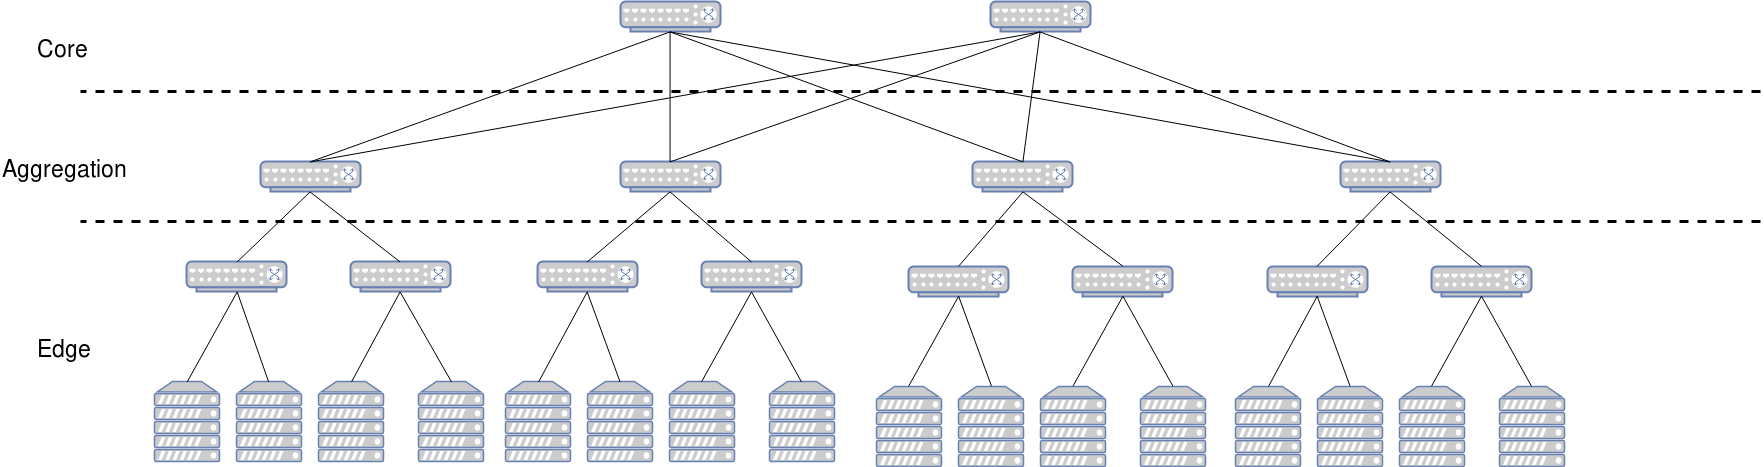
\includegraphics[width=1\textwidth]{nm/fattree}
\caption{Visual representation of the fat tree topology commonly used in data centers}
\end{figure}

A network management system usually consists of a centralized station, and management agents running on the network devices. Using management protocols, the agents can report to the station information about the its operational 
status, which includes information ranging from CPU load to bandwith usage. Typically this information can be retrieved by the controller polling the agents, or the agents sending information on their own, usually to inform
status changes. Using this information, the network operator can get insight on the performance or possible errors of the devices that are monitored. In the next section, we explore one of the most popular management protocols,
SNMP.

\section {SNMP}

The Simple Network Management Protocol is an IETF defined protocol that allows for the interconnection of networking devices, and provide a structured way to retrieve relevant information about these devices. As the name suggests,
SNMP allows for a simplified approach to network monitoring, since it reduces the complexity of the functions that the management agent needs to comply with, which bring several advantages, like reducing
the costs for development of management tools; provides a way to monitor, independently from different hardware providers the resources; and also supports freedom in extending the protocol in order to include other aspects of 
network operation. \cite{CITE - RFC 1157} %% XXX cite https://tools.ietf.org/html/rfc1157
\par  The architectural model of SNMP can be described as the following components:
    
\begin{figure} [h]
    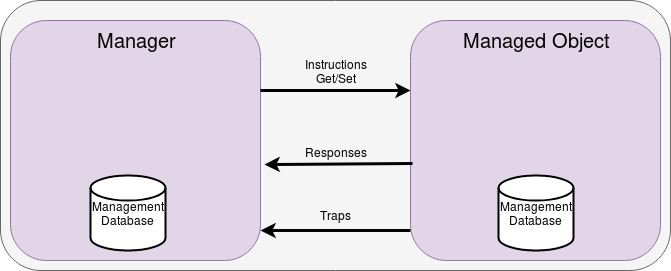
\includegraphics[width=.6\textwidth]{nm/snmp_arch}
    \caption{Architectural components of SNMP}
\end{figure}

The management database is one of the most important components of this system, because it serves as a reference to the entities that are managed in the SNMP protocol. The formal name for this database is the MIB - Management 
Information Base \cite {CITE - RFC 1155}, and its composed of a collection of the objects and their variables. Figure 5.4 features the object groups that make up the MIB. 

\begin{figure} [h]
    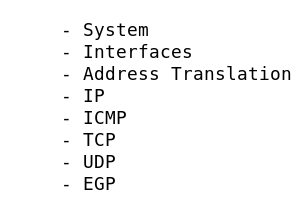
\includegraphics[width=.4\textwidth]{nm/mib_obj}
    \caption{Object groups that compose the MIB \cite{ CITE - RFC 1156}}
\end{figure}

\par The MIB is structured in a tree-like hierarchy. This structure allows for the organization of all objects in a logical pattern, as there is a parent node, that does not have any label, but provides three children, 
that provide different indexes for different organizations, so that each can maintain their own standards. One advantage of this system is that companies can maintain their own MIB, while also remaining compatible with the
rest of the standard. 

\par Due to its permanence in the market, the protocol has suffered some large changes since its original design. SNMPv3 now supports important changes to the original one, most notably in the security aspects, introducing strong
authentication and encryption capabilities.

\section {OpenFlow}

Looking now at OpenFlow related monitoring, some of the 






